\subsection{External Interface Requirements}
\subsubsection{User Interfaces}
The following images represent the mockup of some of the most important pages of the application.\\
\begin{figure}[!htb]

\begin{minipage}[b]{0.4\textwidth}
	\centering
	\includegraphics[scale=0.3]{images/login}
	\caption{Login page}
	\label{ref:login}
\end{minipage}
\hfill
\begin{minipage}[b]{0.4\textwidth}
	\centering
	\includegraphics[scale=0.3]{images/sign-up}
	\caption{Sign up page}
	\label{ref:signup}
\end{minipage}
\end{figure}


\begin{figure}[!htb]

\begin{minipage}[b]{0.3\textwidth}
	\centering
	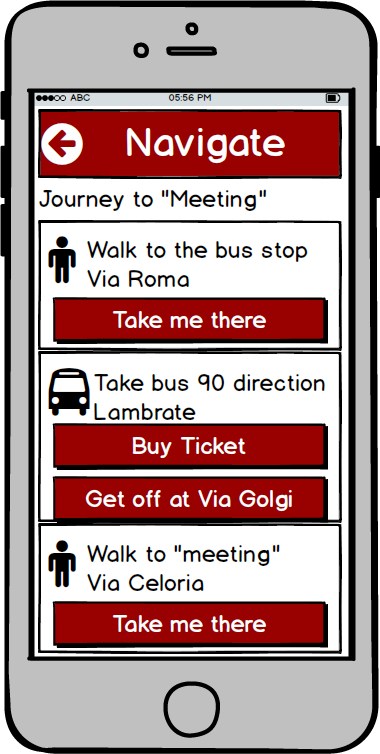
\includegraphics[scale=0.3]{images/Navigate}
	\caption{Navigation page}
	\label{ref:navigate}
\end{minipage}
\hfill
\begin{minipage}[b]{0.3\textwidth}
	\centering
	\includegraphics[scale=0.3]{images/walk}
	\caption{Walking assistant}
	\label{ref:walk}
\end{minipage}
\hfill
\begin{minipage}[b]{0.3\textwidth}
	\centering
	\includegraphics[scale=0.3]{images/bus}
	\caption{Bus assistant}
	\label{ref:bus}
\end{minipage}
\end{figure}

\begin{figure}[!htb]
\begin{minipage}[b]{0.3\textwidth}
	\centering
	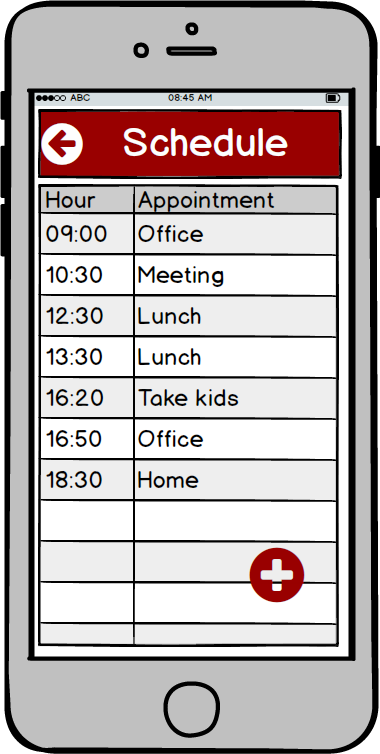
\includegraphics[scale=0.3]{images/Schedule}
	\caption{Schedule page}
	\label{ref:schedule}
\end{minipage}
\hfill
\begin{minipage}[b]{0.3\textwidth}
	\centering
	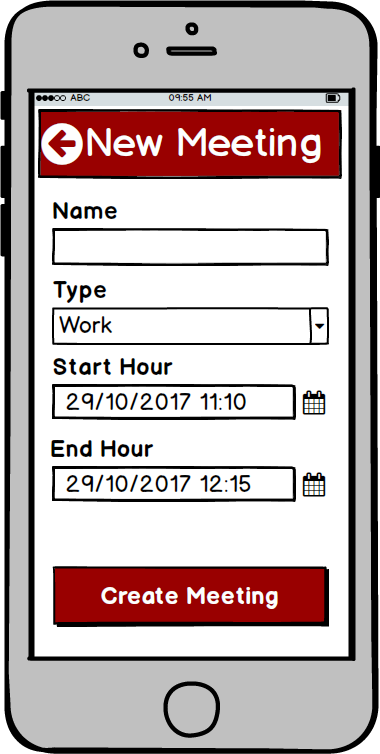
\includegraphics[scale=0.3]{images/NewMeeting}
	\caption{New Meeting}
	\label{ref:newMeeting}
\end{minipage}
\hfill
\begin{minipage}[b]{0.3\textwidth}
	\centering
	\includegraphics[scale=0.3]{images/warning}
	\caption{Warning Pop-up}
	\label{ref:warning}
\end{minipage}
\end{figure}

\begin{figure}[!htb]
\begin{minipage}[b]{0.3\textwidth}
	\centering
	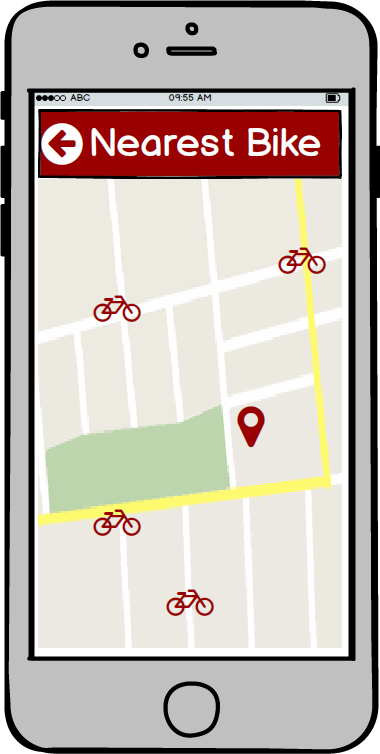
\includegraphics[scale=0.3]{images/SharingSystem}
	\caption{Sharing System}
	\label{ref:shared}
\end{minipage}
\hfill
\begin{minipage}[b]{0.3\textwidth}
	\centering
	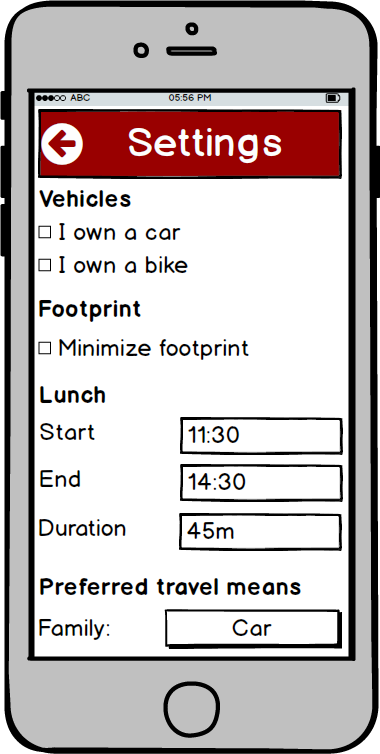
\includegraphics[scale=0.3]{images/Preferences}
	\caption{Preferences Page}
	\label{ref:preferences}
\end{minipage}
\hfill
\begin{minipage}[b]{0.3\textwidth}
	\centering
	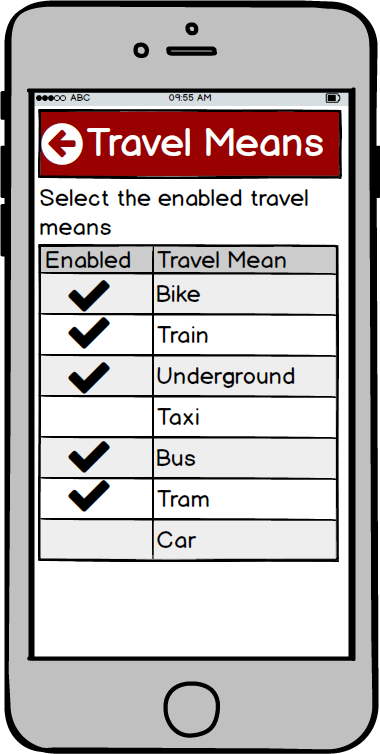
\includegraphics[scale=0.3]{images/TravelMeans}
	\caption{Travel Means}
	\label{ref:travelMeans}
\end{minipage}
\end{figure}

\clearpage
\subsubsection{Hardware Interfaces}
This project doesn't require any hardware interface.

\subsubsection{Software Interfaces}
\renewcommand{\labelitemi}{$\bullet$}
\begin{itemize}
\item Database Management System (DBMS):
	\begin{itemize}
	\item Name: MySQL
	\item Version: 5.6.21
	\item Source: {\href{https://www.mysql.com}		{\color{Black}{https://www.mysql.com}}}
	\end{itemize}
\item Operating System:
	\begin{itemize}
	\item Name: Android
	\item Version: 5.0 Lollipop or higher
	\item Source: {\href{https://www.android.com/}		{\color{Black}{https://www.android.com/}}}
	\end{itemize}
	\begin{itemize}
	\item Name: IOS
	\item Version: 8 or higher
	\item Source: {\href{https://www.apple.com/ios}		{\color{Black}{https://www.apple.com/ios}}}
	\end{itemize} 
\item Application Server:
	\begin{itemize}
	\item Name: Glassfish
	\item Version: 4.1
	\item Source: {\href{https://javaee.github.io/glassfish/}		{\color{Black}{https://javaee.github.io/glassfish/}}}
	\end{itemize}
	
\end{itemize}

\subsubsection{API Interfaces}
For map visualization and to show the track of the journey we use the Google Maps API. This API provides the best and most complete maps system. We can retrieve real time information for road traffic and use these to compute a precise travelling time.\\\\
For the weather information we use the OpenWeatherMap API. This API gives access to current weather data for moreover than 200.000 cities on the world and it takes data from more than 40.000 wheater stations. The data is avaible in various formats: JSON, HTML and XML. We use the 3 hours weather forecasts. For more information see the OpenWeatherMap website ({\href{http://openweathermap.org/api}{\color{Black}{http://openweathermap.org/api}}}).
\\\\
To retrive the information of the schedule and anomalies of train, bus, tram and underground we have an agreement with the companies that provide the services. With this agreement we can use their data to calculate the best track for our users and an advise them when for some reason a service is not avaible.

\subsubsection{Communication Interfaces}
For communications we use the TCP protocol on port 80 for HTTP,port 443 for HTTPS, port 3306 for MySQL database. The data from the server to the application arrive in a JSON format.

\subsection{Scenarios}
\subsubsection{Scenario 1}
Mario is the CEO of a manufacturing company in Milan, his company collaborates with many shops located around in the region. Once a month he must visit each shop to get a report of administrative and management activities. To organize and take into account the travel time for the appointments, he uses Travlendar+. After having downloaded the application and registered his data, Mario has the possibility to create a meeting into the app for every appointment that he has in his personal calendar. During the meeting creation, he needs to specify the following information: location for the meeting, starting and ending time, name and type of the appointment. The app automatically calculates if the time between the end of the first meeting and the start of the second one is enough for the journey; in case the time is too short and the second meeting wouldn't be reachable in time, a warning is shown.

\subsubsection{Scenario 2}
Luca is a young architect of Milan, and in addition to using the latest graphic system to realize his project, he usually produces a demonstration model for his customers scattered around the city. The great capabilities of Luca permits to him to have a lot of appointments, so he uses Travlendar+ to manage the events. Luca has also set the preferences to use car sharing systems for work appointments, in this way he can carry his models around the town without risking of breaking them. The preferences system implemented in the application shows  to the user the best itinerary that respects settings and user's preferences.

\subsubsection{Scenario 3}
Travlendar+ is the perfect application for Giovanni, father of family and financial advisor.
With the application Giovanni can easily manage his travel time to reach every type of appointment. Travlendar+ always suggests to him the perfect way to reach a meeting, in case of work meetings the primary suggestion is public transportation, instead in case of family meetings the primary suggestion is his own car. When Giovanni chooses the public transportations for his movements he can also buy the ticket directly on the app, in a simple way he can select the payment system and in a few taps he can buy it. Furthermore in case of strike the app sends a notification alert to the user and it will recalculate the travel based on the new options.

\subsubsection{Scenario 4}
Antonio is an event organizer and meantime he is a food lover; this is the reason why in his calendar is always presents a lunch in one of the best restaurant of Milan. Antonio is a daily user of Travlendar+ for this reason, the app in fact force a mandatory break of at least 30 minutes for lunch. In this way Antonio can have his lunch break in a period of time between 11.30 am and 2.30 pm and he can arrive in time for the next appointment. Over the lunch break, Antonio usually plans a break in the afternoon, with Travlendar+ he can do this and the minimum time for the break is 5 minutes

\subsubsection{Scenario 5}
Alex is a olympic champion of foot race, when he is not training he is often invited to attend some sport conferences. Alex always suggests that it is really important to do physical activity not only during the training sessions but also when we move around the city. For this reason Alex can not do to use Travlendar+, indeed he chooses the bike for his movements and also selects the option to minimize the carbon footprint. Furthermore the application notifies Alex when the weather conditions are not optimal and suggests him to use another travel mean to reach his desiderated location.


\subsection{Functional Requirements}
 
\subsubsection{Class Diagram}
\begin{figure}[!htb]
\centering
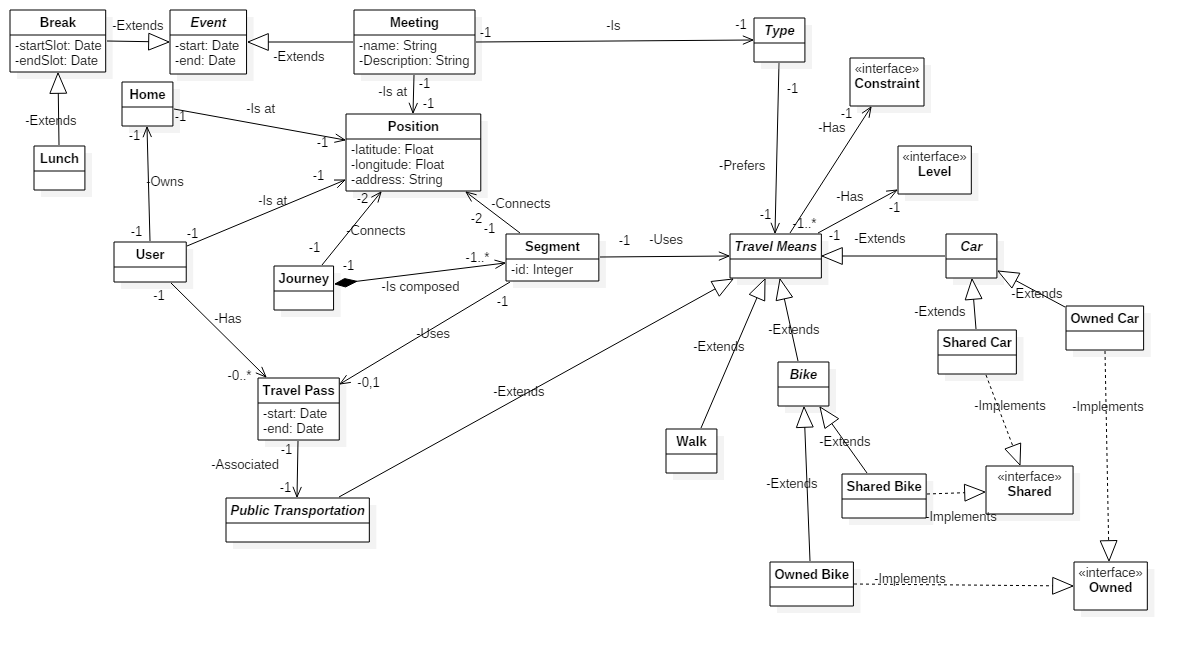
\includegraphics[scale=0.4]{images/ClassDiagram}
\caption{Class Diagram}
\label{ref:classdiagram}
\end{figure}
 
\clearpage
\subsubsection{Use Case Diagram}
\begin{figure}[!h]
\centering
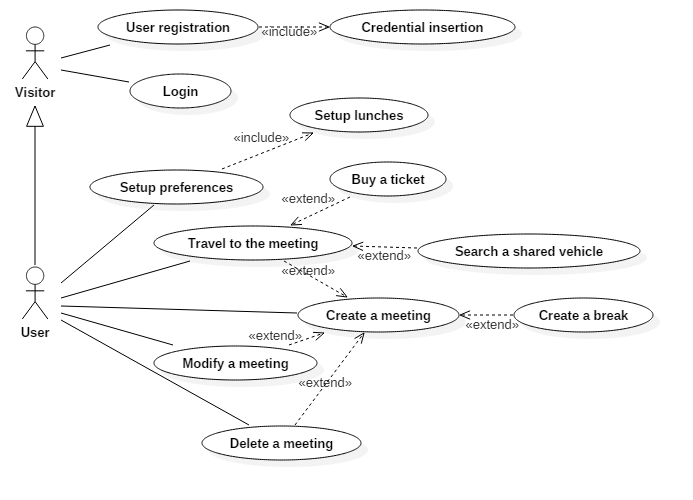
\includegraphics[scale=0.4]{images/UseCaseDiagram}
\caption{Use Case Diagram}
\label{ref:usecasediagram}
\end{figure}
 
\clearpage
\subsubsection{Use Case Descriptions}

In this section are listed some common or significant use cases derivable from
the Use Case diagram.

%Visitor's registration%
\begin{table}
\begin{tabular} { p{5cm} p{8cm} } 
\textbf{Visitor's registration} & \\
\hline
\textbf{Actor:} & Visitor \\ 
\textbf{Goals:} & G.1 \\ 
\textbf{Input conditions:} & The visitor is on the home page. \\
\textbf{Event flow:} & \begin{enumerate}
						\item
						The visitor clicks any button and is redirected to the login page.
						\item
						The visitor clicks on the “Sign Up” button to start the registration process.
						\item
						The visitor fills all the mandatory fields.
						\item
						The visitor clicks on the “Sign Up“ button.
						\item
						The system send the data to the server.
						\item
						The system sends a confirmation email to the new user.
						\end{enumerate}\\ 
\textbf{Output conditions:} & The visitor successfully ends the registration process and is redirected to the login page. From now he can login to the application and start using that. \\ 
\textbf{Exception:} & \begin{enumerate}
						\item
						The visitor is already an user.
						\item
						The visitor inserts not valid information in one or more mandatory fields.
						\item
						The visitor chooses an email that is associated with another user.
						\item
						The server is unreachable.
					\end{enumerate}
All exceptions are handled notifying the issue to the visitor and taking back the Event Flow to the point 2. \\
\hline
\end{tabular}
\caption{Visitor's registration}
\label{ref:visitorsregistration}
\end{table}

%User's login%
\begin{tabular} { p{5cm} p{8cm} } 
\textbf{User's login} & \\
\hline
\textbf{Actor:} & User \\ 
\textbf{Goals:} & G.1 \\ 
\textbf{Input conditions:} & The user is on the login page. \\
\textbf{Event flow:} & \begin{enumerate}
				\item
				The user inserts his credentials into the “email” and “password” fields.
				\item
				The user clicks on the “Login” button in order to access.
			\end{enumerate} \\ 
\textbf{Output conditions:} & The user is successfully redirected to the
home page.\\ 
\textbf{Exception:} & \begin{enumerate}
				\item
				The user inserts a not valid email.
				\item
				The user inserts a not valid password.
				\item
				The server is unreachable.
			\end{enumerate}
All exceptions are handled notifying the issue to the user and taking back the Event Flow to the point 1. \\
\hline
\end{tabular}


%User creates a meeting%
\begin{tabular} { p{5cm} p{8cm} }  
\textbf{Create a meeting}\\
\hline
\textbf{Actor:} & User \\ 
\textbf{Goals:} & G.2, G.3 \\ 
\textbf{Input conditions:} & The user is already logged into the system and is into the schedule page. \\
\textbf{Event flow:} & \begin{enumerate}
				\item
				The user clicks on the “New meeting” button to start the creation process.
				\item
				The user inserts the information  into the fields and the type.
				\item
				The user clicks on the “Create meeting” button.
			\end{enumerate}\\ 
\textbf{Output conditions:} & The user is successfully redirected to the
meeting page.\\ 
\textbf{Exception:} & \begin{enumerate}
				\item
				The name isn’t valid.
				\item
				The start hour doesn’t precede the end hour.
				\item
				The start hour and end hour precede the current date.
				\item
				Exists an another meeting with the same hours. 
				\item
				Travel mean is unavailable. 
			\end{enumerate}
These exceptions are handled notifying the issue to the user and taking back the Event Flow to the point 2.
If the meeting is unreachable, this use case is extended by "Resolve the problem of unreachable meeting".
\\
\hline
\end{tabular}

%Resolve the problem of unreachable meeting%
\begin{tabular} { p{5cm} p{8cm} }  
\textbf{Resolve the problem of unreachable meeting}\\
\hline
\textbf{Actor:} & User \\ 
\textbf{Goals:} & G.2, G.3 \\ 
\textbf{Input conditions:} & The user is creating a meeting and this is unreachable.\\
\textbf{Event flow:} & The applicaiton shows a warning message and the user can either click "Edit" to change the meeting information or click "Create" and continue creating the meeting even if it is unreachable in time.\\ 
\textbf{Output conditions:} & The user is successfully redirected to the
meeting page.\\ 
\textbf{Exception:} & All exceptions are the same as those the use case "Create a meeting". \\
\hline
\end{tabular}

%User travels to the meeting%
\begin{tabular} { p{5cm} p{8cm} }  
\textbf{Travel to the meeting}\\
\hline
\textbf{Actor:} & User \\ 
\textbf{Goals:} & G.4, G.8 \\ 
\textbf{Input conditions:} & The user is already logged into the system and is into the schedule page. \\
\textbf{Event flow:} & \begin{enumerate}
				\item
				The user clicks on the desired meeting and is redirected into the meeting information.
				\item
				The user clicks on “Navigate” and goes into navigate page.
				\item
				The navigate page helps the user with indications.
				\item
				When the user arrives at the desired location, the application notifies him.
			\end{enumerate} \\ 
\textbf{Output conditions:} & The user is successfully redirected to the
schedule.\\ 
\textbf{Exception:} & \begin{enumerate}
				\item
				The GPS is unavailable.
				\item
				Internet connection isn't working.				
				\item
				The location isn’t found. 
			\end{enumerate}
All exceptions are handled notifying the issue to the user and taking back the Event Flow to the point 1. \\
\hline
\end{tabular}


%User selects preferences and filters options%
\begin{tabular} { p{5cm} p{8cm} }
\textbf{Setup preferences} \\
\hline
\textbf{Actor:} & User \\ 
\textbf{Goals:} & G.5, G.7 \\ 
\textbf{Input conditions:} & The user is already logged into the system and is into the home page. \\
\textbf{Event flow:} & \begin{enumerate}
				\item
				The user clicks on “Setting” button and is redirected into setting page.
				\item
				The user inserts his preferences about travel means and lunch timetable.
				\item
				The user confirms the new information with “Confirm” button.
			\end{enumerate}\\ 
\textbf{Output conditions:} & The user stays in the setting page.\\ 
\textbf{Exception:} & \begin{enumerate}
				\item
				The user doesn’t insert numbers in the lunch fields.
			\end{enumerate}
All exceptions are handled notifying the issue to the user and taking back the Event Flow to the point 2. \\
\hline
\end{tabular}


\subsubsection{Sequence Diagrams}


\subsection{Performance Requirements}
\begin{enumerate}
\item
95\% of the requests should be processed within 5 seconds.
\item
100\% of the requests should be processed within 20 seconds.
\item
There is no limit to the total number of the registered users.
\end{enumerate}

\subsection{Design Constraints}

\subsection{Software System Attributes}
\subsubsection{Reliability}
The system is designed to run on a single server and its reliability depends on the server one. The server is required only for logins an backups of the users’ schedules.
In case of downtime, as long as the user is logged in the application, the fault wouldn’t affect the functions and backups would be carried out when the service returns available.

\subsubsection{Availability}
The system is required to have a 99\% uptime. Most scheduled downtimes must occur in the weekends at night time.

\subsubsection{Security}
All the communications between the clients and the server will be encrypted and protected by using the SSL protocol.All attempts of establishing an unsecure communication channel with the server must be refused.
All the information will be stored on the server and security will have high priority; users’ passwords will not be stored in plain text.

\subsubsection{Maintainability}
The code should be documented using JavaDoc in order to enable other developers to easily understand and edit it. The system must provide a configurable logging function for debugging purposes. The development of the software will follow the object-oriented Model-View-Controller pattern and the principles of separation of concerns. The source code management should be done through a Version Control System (e.g. git).

\subsubsection{Portability}
The backend will be developed in Java so that it will be possible to run the application on every machine that supports Java Virtual Machine.
The frontend will be developed in Java for Android and in Swift for iOS and the application must support at least the last three version of each operative system.


